\chapter{Monte Carlo versus closed forms: the benchmark}
\label{cap:benchmark}

In Chapter~\ref{cap:mc} we saw how a Monte Carlo (MC) price is estimated, how its error is measured and how Heston is
simulated. Here we put all of this to the test on cases in which the exact price is known. There are four questions:
\begin{itemize}
\item does the error really fall as $N^{-1/2}$, and how do we check it without fooling ourselves?
\item how much do the variance-reduction techniques (antithetic variates, control variate, quasi-Monte Carlo) gain,
for the same number of scenarios and for the same computing time?
\item how large is the discretization bias of the QE-M scheme at the step used in the project?
\item how do we show that the figures and tables were really produced by the declared code?
\end{itemize}
A single rule runs through the whole chapter: the measurement procedure is fixed \emph{before} looking at the
results, and it is not changed afterwards.

\section{The experimental design}
\subsection{The test cases}
We use three parameter sets (``sets'') and, for each, two contracts: an at-the-money call ($K=F$) and a 90\% put
($K=0.9\,F$). The two strikes of a set are priced on the same paths.

\textbf{The market point.} To tie the benchmark to the data, $F$, $\DF$ and $T$ come from the parity table of Chapter~\ref{cap:dati}: the expiry \mbox{2027-11-19}, the kept expiry closest to one year, with
\[
T=1.034734,\qquad F=7677.961695,\qquad \DF=0.951346 .
\]
Two sets are defined on this point.
\begin{itemize}
\item \textbf{bsm}: Black with constant volatility $\sigma=18.40\%$. It is not a hand-picked number: it is the
at-the-money implied volatility of calibrated Heston at that expiry (COS price at $K=F$, then inverted). The path is
sampled \emph{exactly} in a single step,
\[
\ln\frac{F_T}F=-\tfrac12\sigma^2T+\sigma\sqrt T\,Z,\qquad Z\sim\N(0,1),
\]
so the MC error is noise \emph{only}: there is no discretization bias. Reference: Black-76.
\item \textbf{heston\_cal}: Heston with the calibrated parameters of Chapter~\ref{cap:calibrazione}
($\kappa=4.575$, $\theta=0.0529$, $\xi=1.648$, $\rho=-0.752$, $v_0=0.0524$; Feller violated). QE-M simulation
(Section~\ref{sec:qe-m}) on a uniform grid of $\lceil32T\rceil=34$ steps, that is $\Delta t\le1/32$.
\end{itemize}
The third set is an external anchor:
\begin{itemize}
\item \textbf{heston\_fo}: the Fang and Oosterlee set ($\kappa=1.5768$, $\theta=0.0398$, $\xi=0.5751$,
$\rho=-0.5711$, $v_0=0.0175$) with $F=100$, $\DF=1$, $T=1$ and 32 QE-M steps.
\end{itemize}

\begin{esempio}[title={Example: same ATM vol, very different puts}]
The reference prices are:
\begin{center}
\small
\begin{tabular}{lrr}
\toprule
set & ATM call & 90\% put\\
\midrule
bsm & 544.7286 & 231.8087\\
heston\_cal & 544.7286 & 317.2988\\
heston\_fo & 5.785155 & 2.709532\\
\bottomrule
\end{tabular}
\end{center}
The at-the-money call is identical in the first two sets \emph{by construction}: the $\sigma$ of bsm is precisely the
Heston ATM implied vol. The 90\% put, instead, costs about 37\% more under Heston. This is the skew: with
$\rho=-0.75$ the Heston implied vol at that strike is 21.89\%, against Black's flat 18.40\%. The benchmark therefore
covers both a ``smooth'' case and a case in which the left tail weighs heavily.
\end{esempio}

\subsection{The reference: why COS is ``exact enough''}
Under Heston the reference is the COS method (Chapter~\ref{cap:heston}). But a test ``MC within 3 SE of the
reference'' makes sense only if the error of the reference is \emph{negligible} compared with the SE. Otherwise the
test measures the error of the reference, not that of the MC.

The criterion, fixed in advance, is
\begin{equation}\label{eq:bm-rif}
\max|\text{COS}-\text{Lewis}|\ \le\ 0.01\times\min\SE ,
\end{equation}
where the minimum is taken over all Monte Carlo SEs of the benchmark. The smallest Heston SE is
$3.09\times10^{-3}$, so the threshold is $3.09\times10^{-5}$.

Why three independent methods give confidence:
\begin{itemize}
\item \textbf{COS} expands the density in a cosine series on a truncated interval $[a,b]$; its errors are series and
truncation errors.
\item \textbf{Lewis} integrates the characteristic function along another contour with adaptive quadrature: no
interval, no series.
\item \textbf{Gil-Pelaez} (written by an independent check, with its own code) inverts the two probabilities $P_1$,
$P_2$ separately with an integral over $[0,\infty)$.
\end{itemize}
The numerical errors of the three methods have nothing in common. If they agree, the only thing they share is the
characteristic function, which is in turn checked against published values.

\begin{progetto}[title={In the qpricer project: accuracy of the references}]
\begin{itemize}
\item COS against Lewis: $7.36\times10^{-9}$ at most (heston\_cal, $F=7678$: a relative error of about $10^{-12}$),
$1.9\times10^{-10}$ on the FO set. Threshold $3.09\times10^{-5}$: met with four orders of magnitude to spare.
\item Independent Gil-Pelaez: differs from COS by $7.36\times10^{-9}$ and $1.9\times10^{-10}$, and from Lewis by about
$10^{-12}$.
\item FO set, ATM call: COS $5.785155434$ against the published value $5.785155450$, a gap of $-1.6\times10^{-8}$.
\end{itemize}
The six reference prices are frozen in \path{tests/golden/phase6_benchmark_refs.json}, written by the independent
check with its own Gil-Pelaez.
\end{progetto}

\subsection{Grid, replications and seeds}
\begin{itemize}
\item \textbf{Grid.} $N=2^{10},2^{11},\dots,2^{20}$: 11 points from 1024 to 1{,}048{,}576. Powers of 2 are needed for
Sobol' (Section~\ref{sec:bm-rqmc}).
\item \textbf{Honest counting.} $N$ is always the total number of terminal samples, for \emph{every} method: for
antithetics $N/2$ pairs, for Sobol' 16 nets of $N/16$ points. Only in this way is the comparison ``at equal $N$''
fair.
\item \textbf{Replications.} $R=16$ independent replications for each (set, method, $N$). Replication $r=0$ is the
``single run''.
\item \textbf{Seeds.} The seed of replication $r$ is a fixed formula,
\[
\text{seed}=20261110+10^6\cdot\text{set}+10^5\cdot\text{method}+10^3\cdot i_N+r ,
\]
with set and method numbered in a fixed order. No seed can be chosen after the fact.
\item \textbf{Parallelism.} Each task has its own integer seed, so the results do not depend on the number of
processes used.
\end{itemize}

\section{\texorpdfstring{The $N^{-1/2}$ law}{The N\textasciicircum(-1/2) law}}
\label{sec:bm-pendenza}
\subsection{What is measured: noise and bias kept apart}
The gate of this phase requires the log-log slope of the plain MC error to lie in $[-0.6,-0.4]$. The procedure,
declared before running the full benchmark, is:
\begin{enumerate}
\item OLS regression of $\ln y$ on $\ln N$ over \emph{all} 11 points (no point excluded);
\item $y$ is an \textbf{error metric over the $R=16$ replications}:
\begin{itemize}
\item for bsm, the RMSE against Black: $\mathrm{RMSE}=\sqrt{\tfrac1R\sum_r(\hat V_r-V)^2}$;
\item for Heston, the standard deviation of the replications around their mean (noise only).
\end{itemize}
\end{enumerate}

\begin{perche}[title={Why the bias is removed from the metric for Heston}]
With fixed-step QE-M the expected price is $V+b(\Delta t)$, with $b$ constant in $N$. The RMSE against COS is then
\[
\mathrm{RMSE}(N)\approx\sqrt{b^2+\sigma_g^2/N}\ \xrightarrow{N\to\infty}\ |b| :
\]
for large $N$ the curve flattens onto the bias and the slope tends to zero. The gate would fail for a reason that has
nothing to do with the $N^{-1/2}$ law. The standard deviation of the replications, on the other hand, does not see a
constant added to all prices: it measures only the noise. The bias is measured separately (Section~\ref{sec:bm-bias}).

An independent check verified both things: adding a constant to every price leaves the metric unchanged (identical to
$10^{-9}$), and even when the bias is included (RMSE against its own Gil-Pelaez) the four Heston slopes stay within
the band ($-0.516$, $-0.537$, $-0.520$, $-0.540$), because at the benchmark step the bias is smaller than the SE even
at $N=2^{20}$.
\end{perche}

\subsection{How precise the estimated slope is}
With $R=16$ replications, the RMSE at a given $N$ has a relative error of about $1/\sqrt{2R}\approx18\%$, that is a
noise of about $0.18$ on $\ln y$. The OLS slope has variance $\sigma^2/\sum_j(x_j-\bar x)^2$, with $x_j=\ln N_j$.
The points are equally spaced by $\ln2$ and there are 11 of them, hence
\[
\sum_j(x_j-\bar x)^2=(\ln2)^2\sum_{k=-5}^{5}k^2=110\,(\ln2)^2\approx52.9,
\qquad
\mathrm{sd}(\text{slope})\approx\frac{0.18}{\sqrt{52.9}}\approx0.025 .
\]
The band $[-0.6,-0.4]$ is therefore about 4 standard deviations wide on each side of $-0.5$: correct code misses it
with negligible probability, and a bug that really changes the order of convergence misses it almost always.

\subsection{Why the error of a single run is not fitted}
It is tempting to plot $|\hat V-V|$ of a single run against $N$ and fit the line. It is a bad idea. For one run,
$\hat V-V\approx\SE\cdot Z$ with $Z\sim\N(0,1)$, hence
\[
\ln|\hat V-V|\approx\ln\SE+\ln|Z| .
\]
The term $\ln|Z|$ has variance $\pi^2/8\approx1.23$, that is standard deviation $\approx1.1$: noise of order 1 on
\emph{every} point. Redoing the computation above, the standard deviation of the slope would be about
$1.1/\sqrt{52.9}\approx0.15$, wider than the whole half-band of the gate. The slope of a single run can fall outside
the band with perfect code, or inside it with wrong code. This is why the single-run error is shown in the plots (the
crosses), but never fitted.

\subsection{Why the slope of the SE proves nothing}
The other temptation is to fit the SE estimated by the run: $\SE=s_g/\sqrt N$. But
\[
\ln\SE=\ln s_g-\tfrac12\ln N ,
\]
and $s_g$ converges to $\sigma_g$ with a relative error of order $1/\sqrt{2N}$, which is tiny. The slope is therefore
$-0.5$ \emph{by construction}, for any code that computes a sample standard deviation and divides it by $\sqrt N$.
Even a wrong SE has slope $-0.5$: for example an antithetic SE computed on the $N$ correlated payoffs instead of on the
$N/2$ pair means.

\begin{attenzione}[title={A gate that cannot fail is not evidence}]
In the project the gate fits both quantities, for a total of 12 rows. An independent check pointed out that the 6 SE
rows cannot fail, so the count ``52 gates out of 52'' overstates the evidence. The SE rows remain as a consistency
check; the real evidence comes from:
\begin{itemize}
\item the 6 slopes of the error metric over the replications;
\item 104 slopes recomputed by an independent check with fresh seeds;
\item the \textbf{SE honesty ratio}, $\sqrt{\overline{\text{err}^2}/\overline{\SE^2}}$, which is about 1 only if the
declared SE really is the standard deviation of the error.
\end{itemize}
\end{attenzione}

\subsection{The measured slopes}
\begin{table}[ht]
\centering
\small
\caption{Log-log slopes of plain MC over $N=2^{10}\dots2^{20}$. ``SE'': fit of the SE of run $r=0$ (consistency
check); ``metric'': fit of the error metric over the 16 replications (RMSE for bsm, standard deviation of the
replications for Heston), with the OLS standard deviation.}
\label{tab:bm-pendenze}
\begin{tabular*}{\textwidth}{@{\extracolsep{\fill}}l r r r r@{}}
\toprule
& & & \multicolumn{2}{c}{fresh seeds}\\
\cmidrule(l){4-5}
set and contract & SE & metric & mean $\pm$ sd & trials\\
\midrule
bsm, ATM call & $-0.501$ & $-0.538\pm0.021$ & $-0.509\pm0.023$ & 40\\
bsm, 90\% put & $-0.503$ & $-0.487\pm0.025$ & $-0.503\pm0.029$ & 40\\
heston\_cal, ATM call & $-0.499$ & $-0.517\pm0.022$ & $-0.487\pm0.014$ & 6\\
heston\_cal, 90\% put & $-0.499$ & $-0.554\pm0.020$ & $-0.479\pm0.018$ & 6\\
heston\_fo, ATM call & $-0.505$ & $-0.518\pm0.033$ & $-0.484\pm0.032$ & 6\\
heston\_fo, 90\% put & $-0.500$ & $-0.541\pm0.032$ & $-0.489\pm0.022$ & 6\\
\bottomrule
\end{tabular*}
\end{table}

Table~\ref{tab:bm-pendenze} summarizes the result.
\begin{itemize}
\item The 6 slopes of the error metric range from $-0.554$ to $-0.487$, with OLS standard deviations between 0.020
and 0.033: all within the band, and all compatible with $-0.5$ within about 2.7 standard deviations.
\item An independent check repeated the \emph{same} procedure with fresh seeds, declared in advance: 40 trials for
each bsm strike and 6 for each strike of the two Heston sets, for a total of \textbf{104 slopes}. They range from
$-0.558$ to $-0.445$: none outside the band.
\item The Heston slopes of the project run are all slightly below $-0.5$, those of the check all slightly above. The
difference is about 1.8 standard deviations of a mean over 6 trials, and the check's trials on the two sets share
seeds, so they are correlated: it is not significant.
\end{itemize}

\begin{figure}[p]
\centering
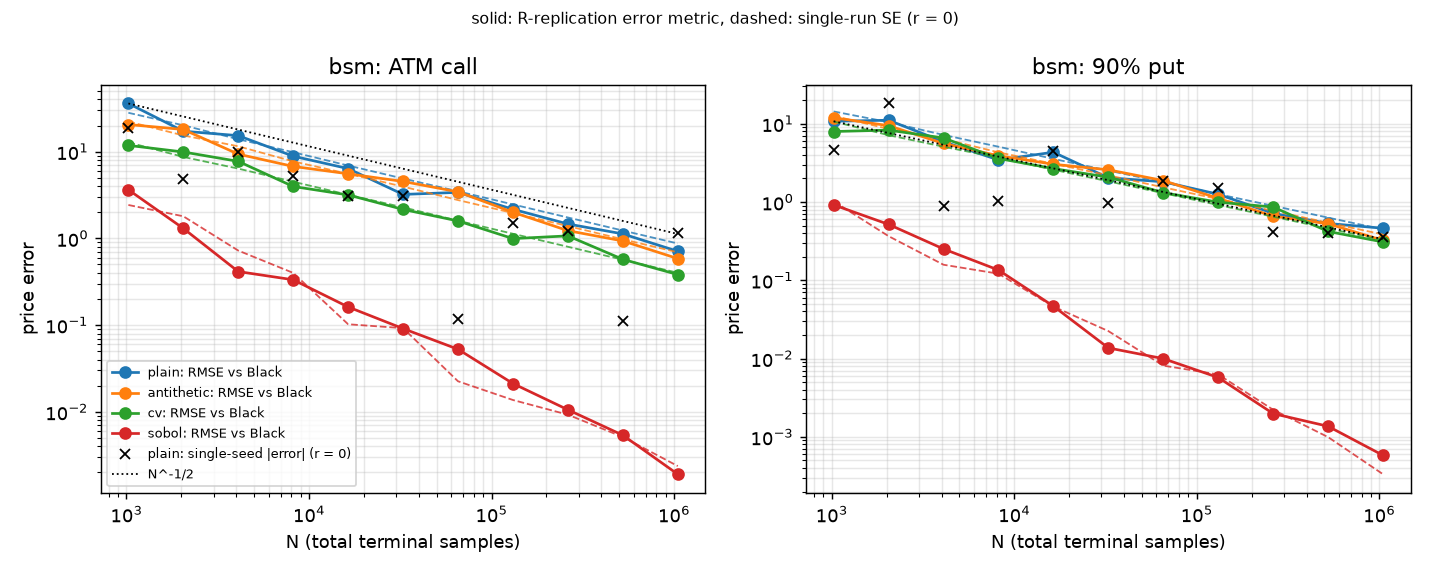
\includegraphics[width=\textwidth]{benchmark_convergence_bsm.png}
\caption{Set bsm: error against $N$ on a log-log scale. Solid lines: RMSE over the 16 replications for each method;
dashed: SE of the single run; crosses: $|\hat V-V|$ of the single plain-MC run; dotted: $N^{-1/2}$ guide.}
\label{fig:bm-conv-bsm}

\bigskip
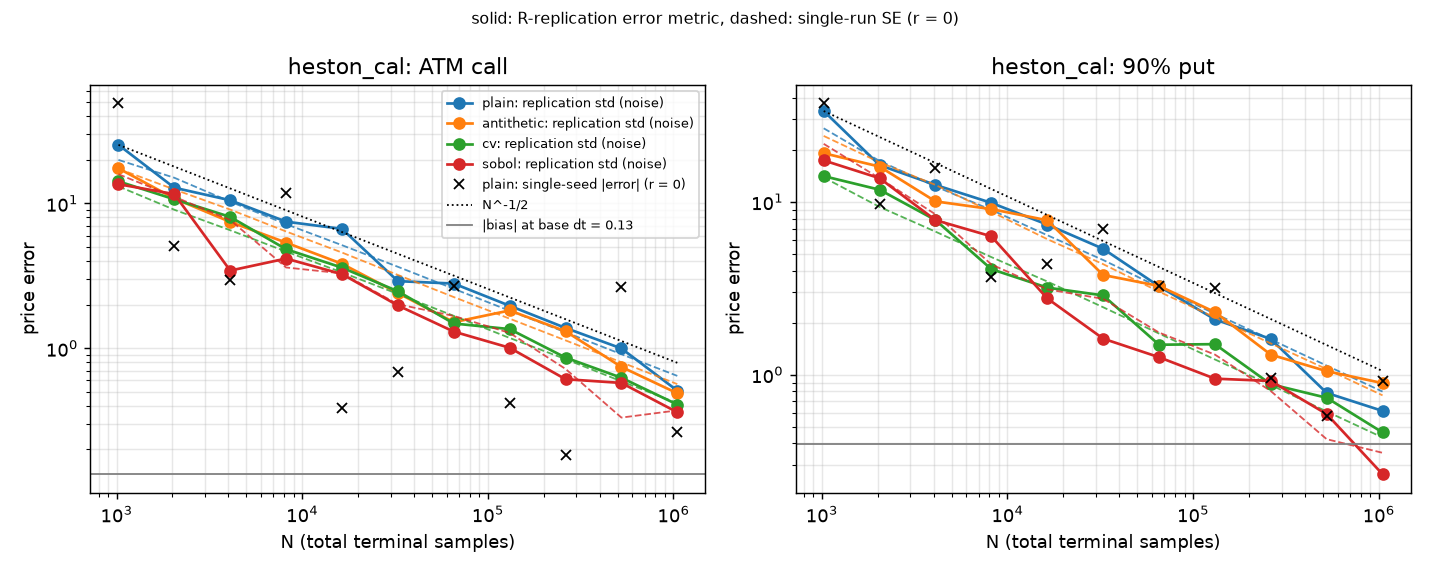
\includegraphics[width=\textwidth]{benchmark_convergence_heston_cal.png}
\caption{Set heston\_cal: as above, but the metric is the standard deviation of the replications (noise only). The
horizontal grey line is the absolute value of the QE-M bias at the benchmark step.}
\label{fig:bm-conv-cal}

\bigskip
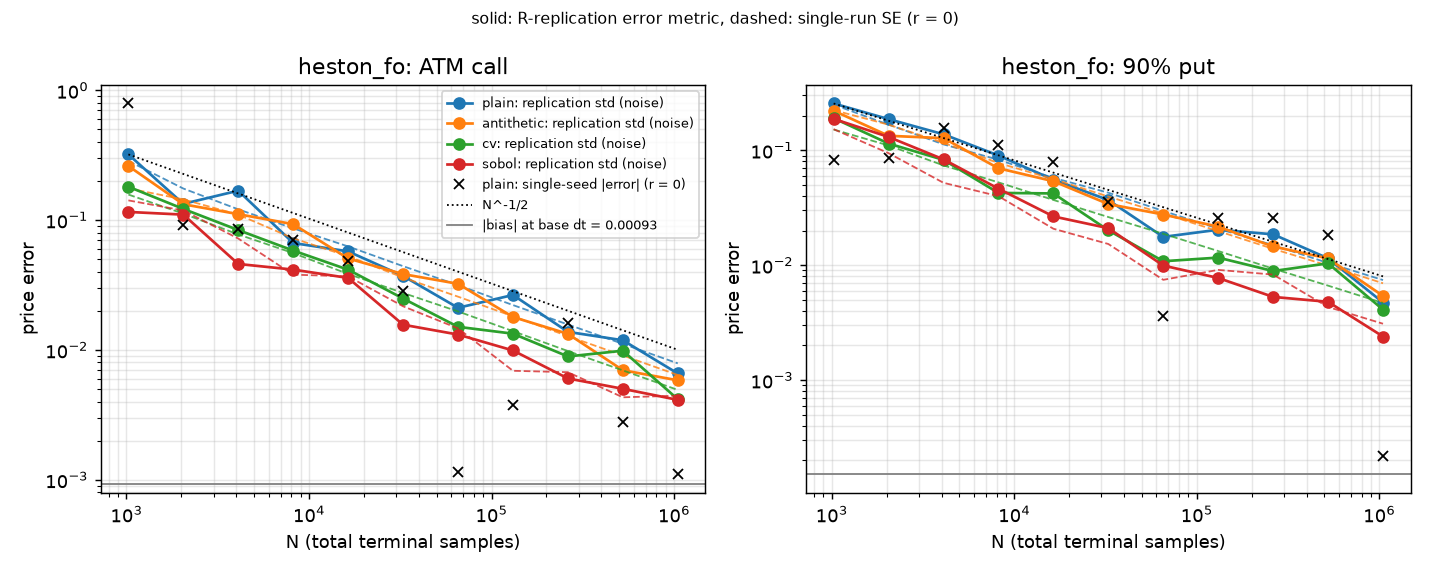
\includegraphics[width=\textwidth]{benchmark_convergence_heston_fo.png}
\caption{Set heston\_fo (Fang--Oosterlee): same legend as Figure~\ref{fig:bm-conv-cal}.}
\label{fig:bm-conv-fo}
\end{figure}

Figures~\ref{fig:bm-conv-bsm}, \ref{fig:bm-conv-cal} and~\ref{fig:bm-conv-fo} show the full curves. Three things to
note.
\begin{itemize}
\item The solid lines of plain, antithetic and control variate are parallel lines of slope $-\tfrac12$: variance
reduction shifts the line down, it does not change its slope.
\item The crosses (error of one run) jump by an order of magnitude from one point to the next: this is the
$\ln|Z|$ noise seen above.
\item Sobol' on bsm (red, Figure~\ref{fig:bm-conv-bsm}) has a clearly steeper slope: it is the only case in which the
method changes the \emph{order} of convergence (Section~\ref{sec:bm-rqmc}).
\end{itemize}

\subsection{The other statistical checks}
\begin{itemize}
\item \textbf{Plain MC within 3 SE at every $N$.} 6 (set, strike) pairs times 11 values of $N$: 66 comparisons, on
run $r=0$. With correct code, by \eqref{eq:test-multipli}, the probability of at least one false alarm is
$1-0.9973^{66}\approx16\%$. The number was written down \emph{in advance}, so that any excursion between 3 and 3.5 SE
would be read as expected multiplicity and not ``fixed'' by changing the seed. Result: $\max|z|=2.90$, none beyond 3.
\item \textbf{Unbiased estimators.} For antithetics, control variate and Sobol' all the $R\times11$ runs are pooled
with weights proportional to $N$:
\[
\bar V=\frac{\sum N\,\hat V}{\sum N},\qquad\SE(\bar V)=\frac{\sqrt{\sum N^2\SE^2}}{\sum N}.
\]
For bsm the comparison is with Black. For Heston it is with plain MC pooled at the same step, with
$\sqrt{\SE_1^2+\SE_2^2}$ in the denominator: this isolates the estimator from the scheme bias, which is the same for
all. 20 comparisons, $\max|z|=2.01$.
\end{itemize}

\section{Variance reduction}
\label{sec:bm-vr}
\subsection{How the methods are compared}
Two measures, both at $N=2^{20}$:
\begin{equation}\label{eq:bm-vr-eff}
\mathrm{VR}_m=\Big(\frac{\overline{\SE}_{\text{plain}}}{\overline{\SE}_m}\Big)^2,
\qquad
\mathrm{eff}_m=\mathrm{VR}_m\times\frac{t_{\text{plain}}}{t_m},
\end{equation}
where $\overline{\SE}$ is the root mean square of the SEs over the replications and $t$ the computing time.
\begin{itemize}
\item $\mathrm{VR}$ says by how much the variance is reduced \emph{for the same number of scenarios}: for the same
error, $\mathrm{VR}$ times fewer scenarios are needed.
\item $\mathrm{eff}$, the work-normalized efficiency, says by how much the variance is reduced \emph{for the same time}. It is the measure that matters
in practice: a method that halves the variance but doubles the time is useless ($\mathrm{eff}=1$).
\end{itemize}
VR could also be defined as the ratio of the replication error metrics. But at a single $N$ that estimate rests on 16
replications: the ratio of two variances with 15 degrees of freedom has a relative error of about $\pm50$--70\%. This
is why the SE-based VR is reported.

\subsection{Antithetic variates}
\textbf{The idea.} If $Z\sim\N(0,1)$, so is $-Z$. One uses $N/2$ normals $Z_j$ and their negatives, and averages the
payoff over the pairs:
\[
h_j=\tfrac12\big[g(Z_j)+g(-Z_j)\big],\qquad\hat V=\DF\,\frac2N\sum_{j=1}^{N/2}h_j .
\]
Under Heston both rows of normals $(Z_v,Z_\perp)$ of each step have their sign flipped.

\textbf{Step 1: the variance.} The $h_j$ are mutually independent, and
\[
\Var h=\tfrac14\big[2\Var g+2\Cov(g(Z),g(-Z))\big]=\tfrac12\Var g\,(1+\rho_A),
\qquad\rho_A=\Corr\big(g(Z),g(-Z)\big).
\]
With $N/2$ pairs, $\Var\hat V=\DF^2\,\Var g\,(1+\rho_A)/N$, hence
\[
\mathrm{VR}=\frac1{1+\rho_A}.
\]
There is a gain only if $\rho_A<0$. If the payoff is even ($\rho_A=+1$, for example a straddle under Black)
antithetics \emph{double} the variance.

\textbf{Step 2: even part and odd part.} Every function can be written as the sum of an odd part and an even part:
\[
g(z)=\underbrace{\tfrac12[g(z)-g(-z)]}_{g_o}+\underbrace{\tfrac12[g(z)+g(-z)]}_{g_e}.
\]
The pair mean is exactly $h=g_e(Z)$: antithetics \emph{cancel the odd part} and leave the even part intact. Since
$g_o$ and $g_e$ are uncorrelated (their product is odd, hence has zero mean),
\[
\mathrm{VR}=\frac{\Var g}{\Var g_e}=1+\frac{\Var g_o}{\Var g_e}.
\]

\begin{perche}[title={Why antithetics help little on convex payoffs}]
For a payoff linear in $Z$ the even part is constant and VR is infinite. An at-the-money call is, to a first
approximation, $\max(z,0)=\tfrac12z+\tfrac12|z|$: half linear (odd, removed) and half ``absolute value'' (even,
surviving). Convexity is precisely the even part, and antithetics do not touch it. For an OTM put the payoff is almost
always zero and the even part weighs even more. The numbers confirm it: under Black VR is 1.59 (ATM call) and 1.35
(90\% put), against the exact values 1.594 and 1.347 computed by an independent check with Gauss--Hermite quadrature.
\end{perche}

\begin{attenzione}[title={Honest counting of the pairs}]
The SE is computed from the $N/2$ pair means, which are independent, \emph{never} from the $N$ payoffs as if they were
independent: they are not. The ``naive'' SE on the $N$ payoffs has an error that depends on the sign of $\rho_A$; in
the project it differs from the correct value by more than 5\%. Above all, it would still have slope $-\tfrac12$: the
slope gate would not notice. In the code (\code{vr.antithetic\_estimate}) an odd $N$ raises an error.
\end{attenzione}

A small practical advantage: antithetics draw half as many normals, so they are also a little faster (under Black
0.0135 s against 0.019 s at $N=2^{20}$). This is why their efficiency exceeds their VR.

\subsection{Control variate: the terminal forward}
Chapter~\ref{cap:asiatiche} derived the control variate \eqref{eq:cv} and the factor $\mathrm{VR}=1/(1-\rho_{XY}^2)$
\eqref{eq:vr}. Here the choice is
\[
Y=\DF\,g(F_T),\qquad X=F_T,\qquad\E X=F .
\]

\textbf{Why the mean is exact.} Under Black the sampling is exact. Under Heston QE-M is used, which is an exact
discrete martingale: $\E[e^{x_{n+1}-x_n}\mid v_n]=1$ at every step (Section~\ref{sec:qe-m}), hence $\E F_T=F$ on any
grid. The control variate therefore adds no discretization bias. With plain QE this would not be so: the spurious
drift of $F_T$ would pass straight into the price. An independent check verified that with QE-M $\overline{F_T}=F$
even at the coarse step $T/9$, with $2^{20}$ paths: $z=-0.10$.

\textbf{The estimated coefficient.} $\hat\beta$ is the OLS slope of $Y$ on $X$ computed on the same paths, and this is
what introduces a small bias. It is computed in three steps. Let $x_i=X_i-F$ and let $e_i$ be the residual of the
population regression, uncorrelated with $x$.

\textit{Step 1.} At first order,
\[
\hat\beta\approx\beta+\frac{\frac1N\sum_ix_ie_i}{\Var X}.
\]

\textit{Step 2.} The estimator is $\hat V=\bar Y-\hat\beta\,\bar x$ and $\E\bar x=0$, so the bias is
\[
\E\hat V-V=-\E[\hat\beta\,\bar x]\approx-\frac{\E\big[\frac1N\sum_ix_ie_i\cdot\frac1N\sum_jx_j\big]}{\Var X}.
\]

\textit{Step 3.} The terms with $i\ne j$ have zero mean (independence and $\E x=0$); the $N$ terms with $i=j$ remain:
\begin{equation}\label{eq:bm-cv-bias}
\E\hat V-V\approx-\frac{\E[x^2e]}{N\Var X}=O\Big(\frac1N\Big).
\end{equation}
The residual is uncorrelated with $x$ but not with $x^2$ (the payoff is convex), so $\E[x^2e]\ne0$. But the bias is
$O(1/N)$, while the SE is $O(N^{-1/2})$: their ratio falls as $N^{-1/2}$.

\begin{progetto}[title={In the qpricer project: the bias of the estimated coefficient}]
Computed by an independent check with a quadrature, under Black:
\begin{itemize}
\item at $N=2^{10}$ the bias is $-0.548$ (ATM call) and $-0.400$ (put), that is 0.043 and 0.031 SE;
\item at $N=2^{20}$ it is $-5.4\times10^{-4}$, that is 0.0013 SE;
\item over 20{,}000 runs at $N=2^{10}$ the mean minus Black matches the predicted bias within 3 SE: there is no other
bias beyond the $O(1/N)$ term.
\end{itemize}
Negligible: to remove it entirely one could estimate $\beta$ on a separate pilot sample, but there is no need.
\end{progetto}

\begin{perche}[title={\texorpdfstring{Why $F_T$ beats the ``shadow Black''}{Why F\_T beats the shadow Black}}]
The alternative considered was the \emph{shadow Black}: the same payoff computed on a Black path driven by the same
normals, with a mean known in closed form (Black-76 at the expected variance). It looks ``closer'' to the payoff, but:
\begin{itemize}
\item with high vol-of-vol ($\xi=1.65$) the Heston log-returns and those of the shadow Black decorrelate, because the
Heston variance moves a lot and that of the shadow does not;
\item $F_T$ is linear and captures the ``delta'' part of \emph{any} payoff, in any model;
\item $F_T$ costs one line of code and is model-independent.
\end{itemize}
Measured on $2^{18}$ paths: VR with $F_T$ equal to 2.39 and 3.41 (heston\_cal, call and put) and 2.56 and 2.51
(heston\_fo), against 1.34, 1.75, 1.74 and 2.39 with the shadow Black. A control variate removes noise, never bias.
\end{perche}

Under Black the exact VR values with $F_T$, computed by an independent check with the partial moments of the
lognormal, are 4.726 (ATM call) and 1.885 (90\% put); the benchmark measures 4.727 and 1.885. The 90\% put is out of
the money: its payoff is zero on most paths and its correlation with $F_T$ is lower.

\subsection{Randomized quasi-Monte Carlo (Sobol')}
\label{sec:bm-rqmc}
\textbf{The idea.} An MC uses random points in $[0,1)^d$, which by chance leave holes and form clumps. A
\emph{quasi}-Monte Carlo uses deterministic \emph{low-discrepancy} points, spread much more evenly. Sobol' sequences
are ``nets'': every elementary box of volume $2^{-m}$ contains exactly the right number of points.

\textbf{Koksma--Hlawka.} For an integrand $f$ of bounded variation $V_{HK}(f)$ (in the sense of Hardy--Krause),
\begin{equation}\label{eq:bm-kh}
\Big|\frac1N\sum_{i=1}^Nf(u_i)-\int_{[0,1)^d}f\Big|\ \le\ V_{HK}(f)\,D_N^*,
\qquad D_N^*=O\Big(\frac{(\log N)^d}{N}\Big),
\end{equation}
where $D_N^*$ is the discrepancy of the points. For small $d$ the error falls almost as $N^{-1}$, much better than
$N^{-1/2}$. But the factor $(\log N)^d$ explodes with dimension, and financial payoffs, after $\Phi^{-1}$, do not have
bounded variation. \eqref{eq:bm-kh} should be taken as intuition, not as a guarantee.

\textbf{Why randomize.} A deterministic net has no standard error: one does not know how wrong one is.
\emph{Scrambling} (random permutations of the binary digits, plus a random digital shift) produces a random net that:
\begin{itemize}
\item preserves the net property (the stratification);
\item has every point, taken on its own, uniform in $[0,1)^d$, so the estimator is unbiased.
\end{itemize}
With 16 \emph{independent} scramblings of $N/16$ points each, the 16 estimates are independent and identically
distributed:
\[
\hat V=\frac1{16}\sum_{q=1}^{16}\hat V_q,\qquad\SE=\frac{s_q}{\sqrt{16}} .
\]
The child seeds are generated with \code{SeedSequence(seed).spawn(16)}. A single net has no error estimate, so no
``3 SE'' test is performed on a single run.

\begin{perche}[title={What splitting the budget into 16 nets costs}]
If the error of a net falls as $c/N$, a net of $N$ points is off by about $c/N$. Sixteen nets of $N/16$ points are
each off by about $16c/N$; the mean of 16 independent errors divides by $\sqrt{16}=4$, leaving $4c/N$. One pays a
factor $\sqrt{16}=4$ on the error, and in exchange obtains a valid SE. With an error that falls only as $N^{-1/2}$ (as
under Heston, see below) the cost disappears.
\end{perche}

\textbf{Dimensions.} Under Black a single normal is needed: $d=1$. Under Heston two normals per step are needed, hence
$d=2\times34=68$ (heston\_cal) and $d=64$ (heston\_fo). Coordinates $(2k,2k+1)$ drive step $k$, in time order, with no
Brownian bridge and no principal components.

\begin{progetto}[title={In the qpricer project: the empirical rate of Sobol'}]
Slope of the replication error metric ($\pm$ OLS standard deviation):
\begin{itemize}
\item \textbf{bsm}: $-1.015\pm0.032$ (ATM call) and $-1.089\pm0.032$ (put). In one dimension a scrambled net is a
stratified sample: for a Lipschitz payoff it would give an RMSE $\propto N^{-1.5}$. But after $\Phi^{-1}$ the payoff is
unbounded or very steep in the boundary cells ($u\to1$ for the call); those cells contribute a variance
$\propto N^{-2}$, hence the slope of about $-1$.
\item \textbf{Heston}: from $-0.51$ to $-0.63$. With 64--68 dimensions ordered in time the \emph{effective dimension}
is high: many coordinates matter, and the stratification in each says little about the payoff. The gain is a constant
factor, not a better order. A Brownian bridge, which puts the large moves of the path in the first coordinates, might
improve the situation; the project does not use one and reports the rate as it is.
\end{itemize}
\end{progetto}

\begin{attenzione}[title={The Sobol' SE is right on average, not in the tails}]
The SE honesty ratio is about 1 for Sobol' too (from 0.95 to 1.04). But an independent check found that the error of
each scrambling is skewed (skewness from $+1.1$ to $+1.7$ under Black): every so often a large positive error,
otherwise small negative errors.
\begin{itemize}
\item \textbf{Why the $t$ statistic has heavy tails.} With a skewed error, the sample mean and the sample standard
deviation of the 16 estimates are correlated. When the rare large error does not occur in the 16 nets, the mean is a
little low \emph{and} the standard deviation is small: $t=(\hat V-V)/\SE$ becomes large and negative.
\item \textbf{How much.} $\PP(|t|>3)$ is between 1.8\% and 3.2\%, against 0.9\% for a Student $t$ with 15 degrees of
freedom and 0.27\% for the normal.
\item \textbf{In the benchmark.} For Sobol' on bsm the mean of $z^2$ is 1.43 and 1.54 (for a $t_{15}$ it would be
1.15), with six runs beyond 3.5 SE, all negative, one as far as $z=-6.17$ (put, $N=2^{17}$). The $z=-2.01$ of the
pooled estimator for the call also comes from here.
\end{itemize}
The conclusion is that the Sobol' SE is calibrated in mean square, but does not license a ``3 SE'' test on a single
run. The cause is the scrambling of a payoff that is unbounded in $u$, not a defect of the code: a second
implementation with different code shows the same effect.
\end{attenzione}

\begin{esempio}[title={Example: the point exactly at zero}]
The library used (\code{scipy.stats.qmc.Sobol}) scrambles 30 binary digits. Every coordinate therefore lies on the
grid $u=k\cdot2^{-30}$, and the value $u=0$ has probability $2^{-30}$ per coordinate. Then $z=\Phi^{-1}(0)=-\infty$.

A full benchmark run draws about $5.3\times10^9$ Sobol' coordinates: the expected number of zeros is
$5.3\times10^9\times2^{-30}\approx4.9$. The first full run did indeed hit $u=0$; the code raised an error, as
designed, and wrote no results.

\textbf{Fix.} The scrambling is completed to full resolution with a uniform inside the point's cell:
\[
u\leftarrow u+U\cdot2^{-30},\qquad U\sim\mathcal U[0,1)\ \text{from the same generator}.
\]
\begin{itemize}
\item \emph{The net stays a net.} Each point stays in its own cell of side $2^{-30}$, so the stratification at every
resolution no finer than $2^{-30}$ is intact (a test checks one point per cell $1/n$).
\item \emph{No bias.} The digital shift makes each coordinate uniform on the grid of $2^{30}$ values; adding a
uniform inside the cell gives exactly $\mathcal U(0,1)$. In fact, the small $O(2^{-30})$ bias of the grid, which
always uses the left end of the cell, disappears.
\item \emph{A check remains.} A coordinate still at 0 or 1 (probability about $2^{-53}$) still raises an error.
\end{itemize}
It is the only change made after a full-run attempt, and it was necessary because that attempt had produced no
output. An independent check used a different fix (53-digit scrambling, no jitter) and obtained statistically
identical results.
\end{esempio}

\subsection{The measured factors}
\begin{table}[ht]
\centering
\small
\caption{Variance reduction at $N=2^{20}$: VR for the same number of scenarios and efficiency for the same time
\eqref{eq:bm-vr-eff}, for the ATM call and the 90\% put. Time: serial median of 3 repetitions, a single machine.}
\label{tab:bm-vr}
\begin{tabular}{llrrrrr}
\toprule
set & method & VR call & VR put & eff call & eff put & time (s)\\
\midrule
bsm & plain & 1 & 1 & 1 & 1 & 0.019\\
& antithetic & 1.59 & 1.35 & 2.24 & 1.89 & 0.014\\
& control $F_T$ & 4.73 & 1.88 & 3.13 & 1.25 & 0.029\\
& Sobol' & $1.4\cdot10^5$ & $7.5\cdot10^5$ & $1.6\cdot10^5$ & $8.4\cdot10^5$ & 0.017\\
\midrule
heston\_cal & plain & 1 & 1 & 1 & 1 & 1.34\\
& antithetic & 1.30 & 1.11 & 1.43 & 1.22 & 1.21\\
& control $F_T$ & 2.39 & 3.42 & 2.21 & 3.16 & 1.44\\
& Sobol' & 3.34 & 6.78 & 2.35 & 4.78 & 1.90\\
\midrule
heston\_fo & plain & 1 & 1 & 1 & 1 & 1.28\\
& antithetic & 1.51 & 1.13 & 1.54 & 1.16 & 1.25\\
& control $F_T$ & 2.56 & 2.50 & 2.49 & 2.44 & 1.32\\
& Sobol' & 4.57 & 5.97 & 3.10 & 4.05 & 1.89\\
\bottomrule
\end{tabular}
\end{table}

Table~\ref{tab:bm-vr} summarizes the results.
\begin{itemize}
\item \textbf{Under Black} Sobol' dominates by five orders of magnitude: it is the one-dimensional case, where the
order of convergence changes. Among the ``classical'' methods the control variate wins on the ATM call (VR 4.73),
while on the OTM put the control reduces the variance more (VR 1.88 against 1.35), but antithetics take less time and
win on efficiency (1.89 against 1.25).
\item \textbf{Under Heston} the gains are modest factors. The $F_T$ control variate gives VR between 2.4 and 3.4 at the
cost of 3--8\% more time; Sobol' gives VR between 3.3 and 6.8 but costs 42--48\% more time, so its efficiency drops to
2.3--4.8. Antithetics give little (VR 1.11--1.51), as expected for convex payoffs.
\item \textbf{Combinations.} The methods were not combined (for example Sobol' with the $F_T$ control): the benchmark
compares them one at a time.
\end{itemize}

\begin{figure}[ht]
\centering
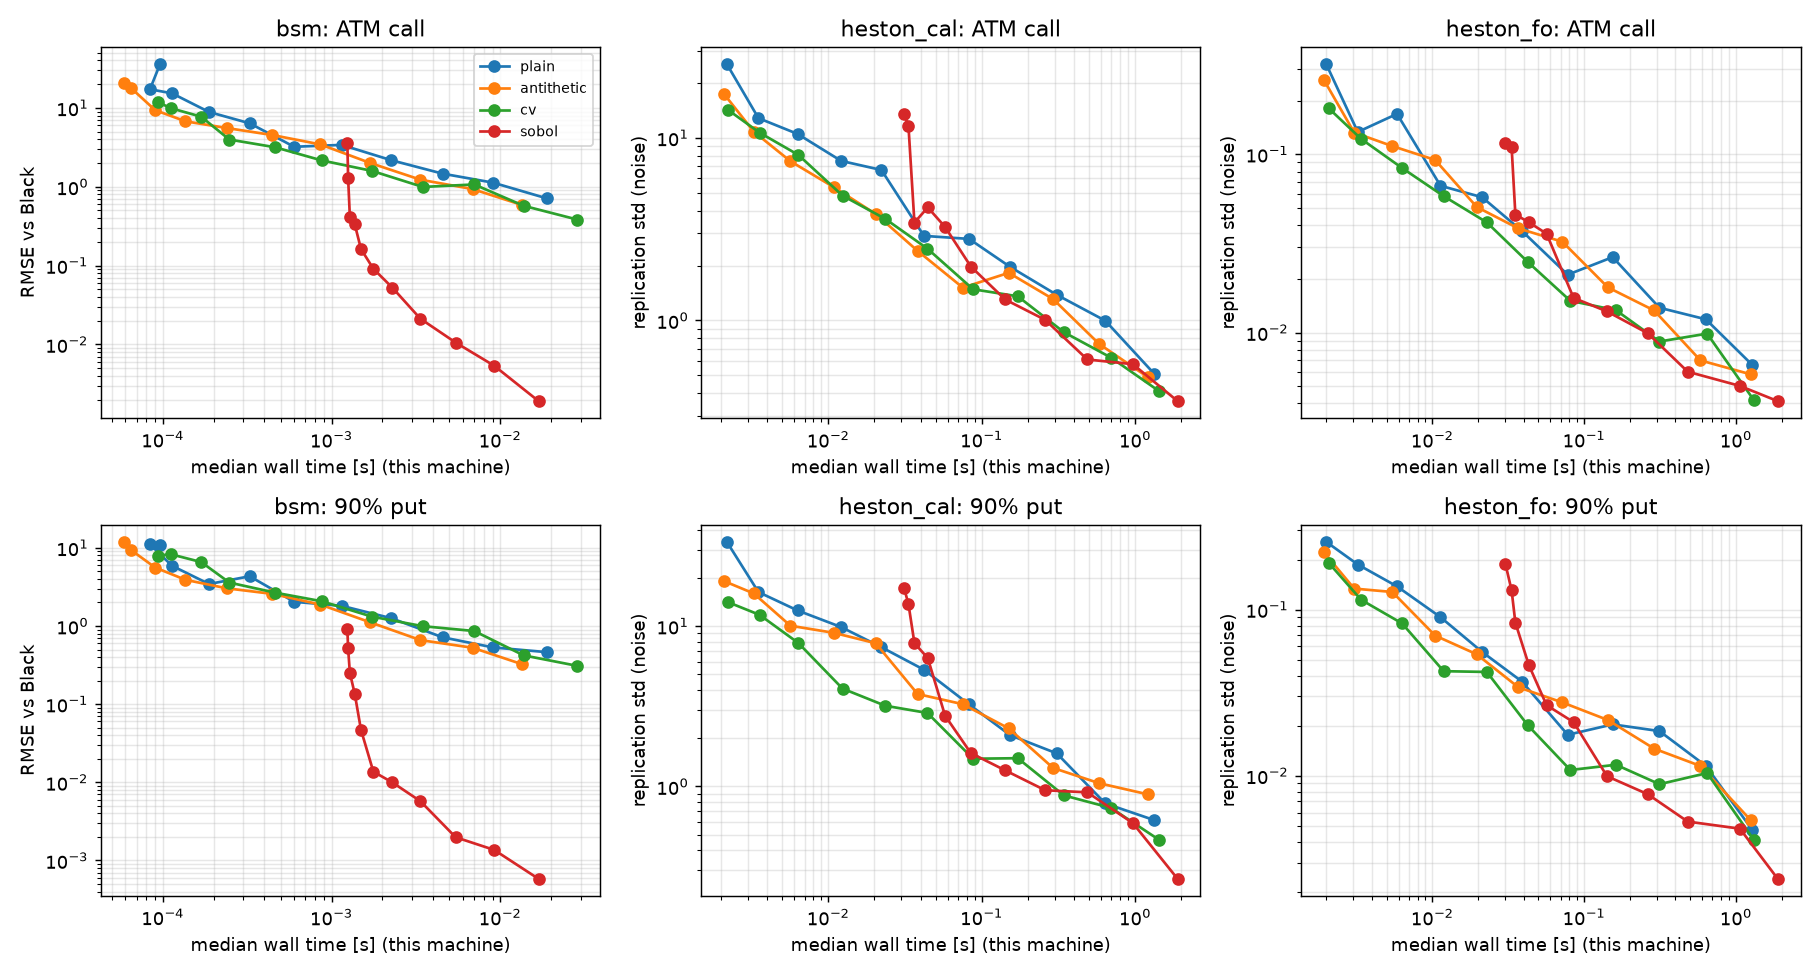
\includegraphics[width=\textwidth]{benchmark_time_vs_error.png}
\caption{Error (RMSE for bsm, standard deviation of the replications for Heston) against median computing time, for
the four methods, on a log-log scale. Times measured on a single machine.}
\label{fig:bm-tempo}
\end{figure}

Figure~\ref{fig:bm-tempo} plots the error as a function of time instead of $N$: it is the ``equal work'' comparison.
The almost vertical stretch of the Sobol' curve on the left has a trivial explanation: for small $N$ the time is
dominated by the construction of the 16 Sobol' generators (about 1 ms), not by the payoff computation.

\needspace{9\baselineskip}
\begin{attenzione}[title={Timings hold for one machine}]
The timings are serial medians on a single laptop, with the installed NumPy version: only the \emph{ratios} between
methods make sense off that machine. Even so they are noisy. Repeating the whole benchmark on the same machine, the
Heston efficiencies move by less than 10\%. Those of bsm move by 9--22\% (Sobol' $-22\%$), because the Black timings
are 14--29 milliseconds in this run (11--29 across runs) and are affected by every disturbance. The bsm efficiencies
should be read as indicative. The VRs, instead, depend only on the seeds and are bit-for-bit reproducible.
\end{attenzione}

\section{The QE-M discretization bias}
\label{sec:bm-bias}
\subsection{How it is measured}
The bias is the difference between the expected value of the scheme at a given step and the exact price:
$b(\Delta t)=\E\hat V_{\Delta t}-V_{\text{COS}}$. To see it, an SE much smaller than that of the benchmark is needed.
The procedure, declared in advance:
\begin{itemize}
\item estimator with the $F_T$ control variate (no additional bias, because QE-M is a martingale);
\item $8\times2^{20}\approx8.4\times10^6$ paths per level;
\item four steps: the base step times $\{\tfrac14,\tfrac12,1,2\}$, rounded up. For heston\_cal they are 9, 17, 34 and
68 steps; for heston\_fo 8, 16, 32 and 64;
\item the bias is also reported in \textbf{vol basis points} (1 bp $=0.01$ vol points), dividing by the Black vega at
the COS implied vol: about 0.295 per bp on the ATM call and 0.25 on the put.
\end{itemize}

\subsection{The full ladder}
On the heston\_cal set the same measurement was redone by an independent check with its own QE-M implementation; the
two estimates agree within 1.85 SE at all 8 points. Table~\ref{tab:bm-bias} reports the combined estimate of the two
runs.

\begin{table}[ht]
\centering
\small
\caption{QE-M bias on heston\_cal, $\hat V_{\Delta t}-V_{\text{COS}}$: combined estimate of the two independent runs,
in price units and in vol basis points. At step $T/17$ the put is about $-7$ SE.}
\label{tab:bm-bias}
\begin{tabular}{l r r r r}
\toprule
& \multicolumn{2}{c}{ATM call} & \multicolumn{2}{c}{90\% put}\\
\cmidrule(lr){2-3}\cmidrule(l){4-5}
$\Delta t$ & price & vol bp & price & vol bp\\
\midrule
$T/9$ & $+2.16\pm0.10$ & $+7.3$ & $+0.37\pm0.11$ & $+1.5$\\
$T/17$ & $+0.03\pm0.10$ & --- & $-0.80\pm0.11$ & $-3.2$\\
$T/34$ (benchmark) & $-0.17\pm0.10$ & $-0.6$ & $-0.40\pm0.11$ & $-1.6$\\
$T/68$ & $-0.23\pm0.10$ & $-0.8$ & $-0.28\pm0.11$ & $-1.1$\\
\bottomrule
\end{tabular}
\end{table}

\begin{figure}[ht]
\centering
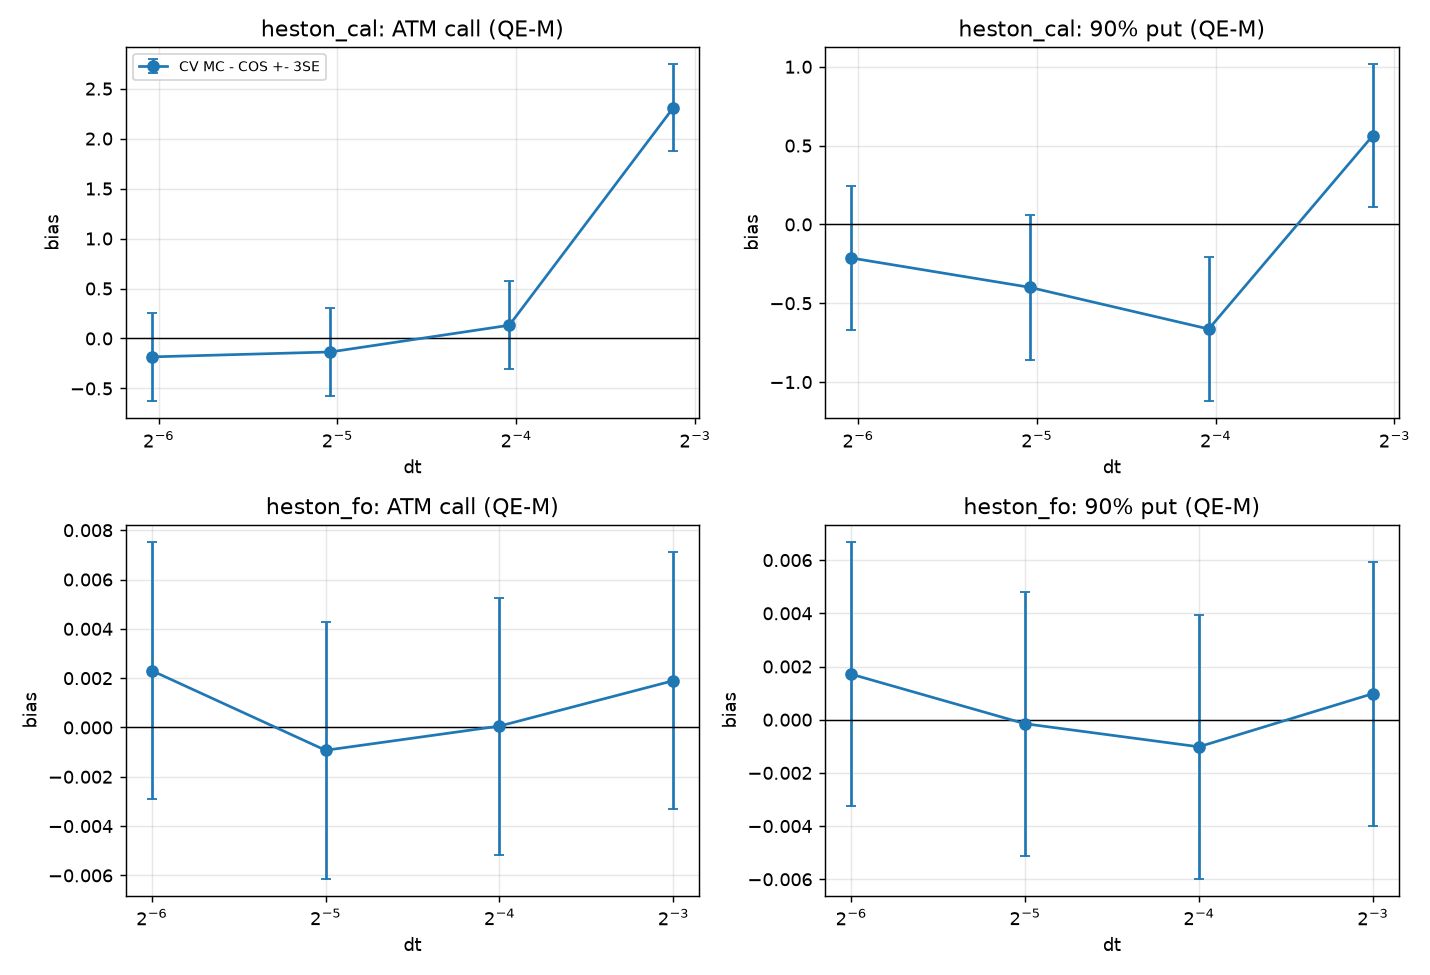
\includegraphics[width=0.9\textwidth]{benchmark_heston_bias.png}
\caption{QE-M bias (control-variate MC minus COS, bars $\pm3$ SE) against the step $\Delta t$, project run. Top:
heston\_cal, bottom: heston\_fo; left: ATM call, right: 90\% put.}
\label{fig:bm-bias}
\end{figure}

Table~\ref{tab:bm-bias} and Figure~\ref{fig:bm-bias} read as follows.
\begin{itemize}
\item \textbf{At the benchmark step ($T/34$)} the bias is small: $-0.6$ bp on the call and $-1.6$ bp on the put. Over
the whole fine ladder ($T/17$, $T/34$, $T/68$) it stays within about 3 bp. It is also smaller than the plain-MC SE at
$N=2^{20}$ (0.64 on the call, 0.80 on the put): it therefore cannot distort a 3 SE test on a single run. It becomes
visible only at the precision pooled over all replications: pooled plain MC minus COS is $-0.29$ ($-2.5$ SE) on the
call and $-0.30$ ($-2.1$ SE) on the put, over about $3.4\times10^7$ paths. This is precisely why the slope gate uses
the noise-only metric.
\item \textbf{At the coarse step $T/9$} the bias on the ATM call is large: $+2.31$ in the project run (15.9 SE,
$+7.8$ bp), $+2.02$ in the independent run, $+7.3$ bp combined. The step ($\Delta t\approx0.115$) is about half the
mean-reversion time $1/\kappa\approx0.22$, and with $\xi=1.65$ the variance moves a lot within a single step.
\item \textbf{The put is not monotonic in $\Delta t$}: $+0.37$, $-0.80$, $-0.40$, $-0.28$ as the step is halved. The
QE-M bias is not a simple $c\,\Delta t$ like that of Euler (Chapter~\ref{cap:mc}): it can change sign. The halving
differences between $T/17$, $T/34$ and $T/68$ stay within 1.3 SE, but this alone would hide the shape of the curve:
this is why the full ladder is reported.
\item \textbf{A non-robust point.} The put value at $T/9$ is $+0.56$ (3.7 SE) in the project run and $+0.17$ (1.1 SE)
in the independent one. Taken on its own, it is not a result.
\item \textbf{Set heston\_fo}: every level is within 1.33 SE of COS ($|b|\le0.0023$ on a price of 5.79). With
$\xi=0.58$ and Feller less violated the scheme is already exact within the noise at 8 steps.
\end{itemize}

\begin{idea}[title={Key idea: two errors, two measurements}]
Noise and bias are measured with different tools. Noise is measured from the dispersion of the replications and falls
as $N^{-1/2}$. Bias is measured with many more paths, at several steps, against an exact reference, and does not
depend on $N$. Mixing them in a single ``error against $N$'' curve makes the bias look like a slowdown of convergence.
\end{idea}

\section{Reproducibility}
\subsection{Deterministic regeneration}
All the figures and tables of the benchmark (the \path{benchmark_*} files in \path{report/figures/}) are written by a
single script, \path{scripts/run_benchmarks.py}. The script also writes a \emph{manifest}
(\path{benchmark_manifest.csv}) with, for each file: the sha256 hash, the size, the script that wrote it, the time of
the run and the configuration (``full'' or ``quick''). The reproducibility gate checks that:
\begin{itemize}
\item every listed file exists and has the recorded hash (12 files out of 12);
\item the configuration is the full one;
\item there are no unlisted \path{benchmark_*.png} figures (0 stray files).
\end{itemize}

\begin{attenzione}[title={Integrity is not provenance}]
The manifest is written by the very script one wants to verify, and the ``written by'' field is a string. A matching
hash only shows that the files have not changed \emph{after} the run (integrity). It does not show that they were
produced by that code (provenance).

Provenance is shown in another way: by re-running. An independent check re-ran the whole \path{run_benchmarks.py} in
a separate folder, with 6 processes instead of 8 (218 s). Result:
\begin{itemize}
\item bit-for-bit identical: the three convergence figures, the bias figure, and the tables of references,
convergence, bias and control choice;
\item in the table of runs, every price and every SE bit-for-bit identical; only the timings change;
\item different, as expected, only the outputs that depend on timings: the time--error figure, the timing table and
the time and efficiency columns of the summary.
\end{itemize}
The project's two full runs (216 s and 294 s, different machine load) also have bit-for-bit identical prices and SEs.
\end{attenzione}

\subsection{Declared in advance, but how do we know?}
The procedure (cases, grid, replications, seeds, metrics, gates) was written before the full run. But it was committed
to version control together with the results, so the repository history alone does not prove it. That there was no
selection is shown by three facts:
\begin{itemize}
\item the procedure leaves nothing to choose: all 11 points, all 6 pairs, both fits, a fixed formula for the seeds;
\item with fresh seeds, 0 slopes out of 104 fall outside the band, with standard deviations (0.014--0.032) much
smaller than the half-width of the band (0.1);
\item the independent re-run is bit-for-bit identical.
\end{itemize}

\begin{progetto}[title={In the qpricer project: the benchmark files}]
\begin{itemize}
\item \path{src/qpricer/engines/vr.py}: the function \code{vanilla\_mc}, which implements the four methods
(\code{plain}, \code{antithetic}, \code{cv} and \code{sobol}), plus the helper functions for the antithetic pairs and
for the Sobol' normals. Every pricer returns \code{(price, SE, N, seed)}.
\item \path{scripts/run_benchmarks.py}: cases, references, parallel runs, serial timing pass, bias and control-choice
studies, figures and manifest. The \code{-{}-quick} option runs a minimal grid for the tests.
\item \path{scripts/phase6_gates.py}: the 52 checks, read from the files on disk.
\end{itemize}
\end{progetto}

\begin{riassunto}
\begin{itemize}
\item Benchmark on an SPX point close to one year (Black at the Heston ATM vol, calibrated Heston) and on the
Fang--Oosterlee set; COS reference, checked against Lewis and independent Gil-Pelaez to better than $10^{-8}$.
\item $N^{-1/2}$ slope: fit a metric over the replications (RMSE, or the dispersion for Heston, to exclude the bias),
never the error of one run (too noisy) nor the SE (slope $-0.5$ by construction). Measured: from $-0.554$ to $-0.487$;
104 trials with fresh seeds between $-0.558$ and $-0.445$.
\item Antithetics: VR $=1/(1+\rho_A)$, they remove the odd part of the payoff and leave the convexity; SE from the
pairs. $F_T$ control: exact mean even under QE-M, bias of the estimated $\hat\beta$ $O(1/N)$, better than the shadow
Black. Randomized Sobol': order about $N^{-1}$ in one dimension, only a constant factor at 64--68 dimensions; SE from
16 scramblings, right on average but with heavy tails.
\item For the same time, under Heston: $F_T$ control 2.2--3.2, Sobol' 2.3--4.8, antithetics 1.2--1.5.
\item QE-M bias at step $T/34$: $-0.6$ and $-1.6$ bp; at $T/9$ up to $+7.3$--$7.8$ bp on the ATM call; non-monotonic
on the put.
\item The sha256 manifest proves integrity; the bit-for-bit identical independent re-run proves provenance.
\end{itemize}
\end{riassunto}

\begin{domande}
\begin{enumerate}
\item Why does the slope gate for Heston use the standard deviation of the replications and not the RMSE against COS?
\item Why is the slope of the error of a single run too noisy for a gate? Roughly what is its standard deviation over
11 points?
\item Why is the slope of the SE $-0.5$ even for wrong code? Which check does have power?
\item Show that antithetics have $\mathrm{VR}=1+\Var g_o/\Var g_e$. When do they make things worse?
\item Why does the $F_T$ control variate introduce no discretization bias under QE-M? What would happen with plain QE?
\item Where does the $O(1/N)$ bias of the estimated coefficient come from, and why is it negligible?
\item Why does Sobol' converge at about $N^{-1}$ under Black and almost at $N^{-1/2}$ under Heston?
\item Why does the $t$ statistic of the 16 scramblings exceed 3 more often than expected? What does this imply for the
tests?
\item Why does adding a uniform inside the $2^{-30}$ cell neither introduce bias nor break the net?
\item What is the difference between the integrity and the provenance of a result? What does each one prove?
\end{enumerate}
\end{domande}
